
\section{Efficiency}
\label{sec:efficiency}

Though it is a single board, the Raspberry Pi operates more like a computer than an integrated circuit. It most commonly runs a custom Linux distribution, Raspbian, allowing Autopilot to use Python across the whole system. Using an interpreted language like Python running on Linux has inherent performance drawbacks compared to compiled languages running on embedded microprocessors. While Python's overhead is negligible on modern processors, Autopilot is nevertheless designed to maximize computational efficiency.

\subsection{Concurrency}

\begin{marginfigure}[3.5cm]
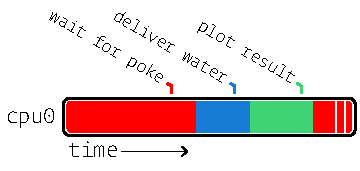
\includegraphics[]{figures/side_12_onethread.pdf}
\caption{A single-threaded program executes all operations sequentially, using a single process and cpu core.}
\label{fig:singlethread}
\end{marginfigure}

Most behavioral software is single-threaded (Figure \ref{fig:singlethread}), meaning the program will only perform a single operation at a time. If the program is busy or waiting for an input, other operations are blocked until it is finished.

Autopilot distributes computation across multiple processes and threads to take advantage of the Raspberry Pi's four CPU cores. Every object in Autopilot does its work in separate \textbf{threads}. Specifically, Autopilot spawns separate threads to process messages and events, an architecture described more fully in \hyperref[sec:networking]{section \ref*{sec:networking}}. Threading does not offer true concurrency\sidenote{See David Beazley's  \href{http://www.dabeaz.com/python/UnderstandingGIL.pdf}{'Understanding the Global Interpreter Lock'} and associated \href{http://www.dabeaz.com/GIL/gilvis/index.html}{visualizations}.}, but does allow Python to distribute computational time between operations so that, for example, waiting for an event does not block the rest of the program, and events are not missed because the program is busy (Figure \ref{fig:multithread}).

\begin{marginfigure}
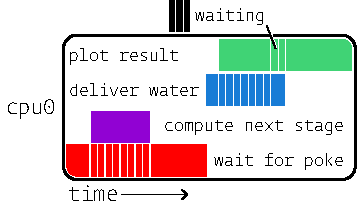
\includegraphics[]{figures/side_13_multithread.pdf}
\caption{A multi-threaded program divides computation time of a single process and cpu core across multiple operations so that, for example, waiting for input doesn't block other operations.}
\label{fig:multithread}
\end{marginfigure}

Critical operations that are computationally intensive or cannot be interrupted are given their own dedicated \textbf{processes}. Linux allows individual cores of a processor to be reserved for single processes, so individual Raspberry Pis are capable of running four truly parallel processing streams. For example, all Raspberry Pis in an Autopilot swarm create a messaging client to handle communication between devices which runs on its own processor core so no messages are missed. Similarly, if an experiment requires sound delivery, a realtime \hyperref[sec:stim]{sound engine} in a separate process (Figure \ref{fig:multiprocess}) also runs on its own core.

\begin{marginfigure}[0.1cm]
 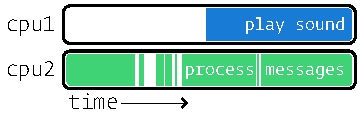
\includegraphics[]{figures/side_14_multiprocess.pdf}
 \caption{A multi-process program is truly concurrent, allowing multiple cpu cores to operate in parallel.}
 \label{fig:multiprocess}
\end{marginfigure}

\subsection{Leveraging Low-Level Libraries}
\label{sec:lowlevel}

Autopilot uses Python as a "glue" language, where it wraps and coordinates faster low-level compiled code\citep{vanrossumGlueItAll1998}.  
Performance-critical components of Autopilot are thin wrappers around fast C libraries (Table \ref{tab:libraries}).

\begin{margintable}[0.1cm]
\caption{A few libraries Autopilot uses}
\label{tab:libraries}
\noindent\begin{tabularx}{\linewidth}{Rl}
\toprule
 \textbf{\href{http://jackaudio.org/}{jack}} & realtime audio \\
 \textbf{\href{http://abyz.me.uk/rpi/pigpio/index.html}{pigpio}} & GPIO control \\
 \textbf{\href{http://zeromq.org/}{ZeroMQ}} & networking \\
 \textbf{\href{https://www.qt.io/}{Qt}} & GUI \\
 \bottomrule
\end{tabularx}

\end{margintable}

Since Autopilot coordinates its low-level components in parallel rather putting everything inside one "main loop," Autopilot actually has \textit{better} temporal resolution than  single-threaded systems like Bpod or pyControl, despite the realtime nature of their dedicated processors (Table \ref{tab:precision}).

\begin{margintable}
\caption{Using pigpio as a dedicated I/O process gives autopilot greater measurement precision}
\label{tab:precision}
\noindent\begin{tabularx}{\linewidth}{rR}\toprule
& Precision \\
\midrule
Autopilot (\href{http://abyz.me.uk/rpi/pigpio/pigpiod.html}{pigpio}) & $5\mu s$ \\
\href{https://github.com/sanworks/Bpod_StateMachine_Firmware/blob/059d1e9195f5bb7d0d5cd7b33f56342eb5a3a55c/Dev/StateMachineFirmware/StateMachineFirmware.ino\#L196}{Bpod} & $100\mu s$ \\
\href{https://bitbucket.org/takam/pycontrol/src/c678552ac57be2108a5461e0c5f8051ce7d3816a/pyControl/framework.py?at=default\&fileviewer=file-view-default\#framework.py-278}{pyControl} & $1000\mu s$ \\
\bottomrule
\end{tabularx}

\end{margintable}

\subsection{Caching}

Finite-state machines are only aware of the current state and the events that transition it to future states. They are thus incapable of exploiting the often predictable structure of behavioral tasks to precompute future states and precache stimuli. Further, to change task parameters between trials (eg. changing the rewarded side in a two-alternative forced-choice task), state machines need to be fully reconstructed and reuploaded to the device that runs them each time.

Autopilot precomputes and caches as much as possible. Rather than wait "inside" a state, Autopilot prepares each of the next possible events and saves them for immediate execution when the appropriate trigger is received. Static stimuli are prepared once at the beginning of a behavioral session and stored in memory. Before their presentation, they are buffered to minimize latency.

\vspace{16pt}

Autopilot's efficient design lets it access the best of both worlds---the speed and responsiveness of compiled code on dedicated microprocessors and the accessibility and flexibility of interpreted code.